% \section{First principles model}
% \label{sec:first_principles_model}
% \todo[inline]{Introduction}
% Modelling the underlying chemical and thermal processes can be very challenging, because of the wide variety in waste-composition, as described in \cite{waste_prof}. The waste will often be an inhomogeneous mix with different moisture-levels, heat conductivity and absorption/emission-factors, that may change as the waste burns. The primary goal of the regulator is to avoid the sudden spikes in $NO_x$, $CO$ and $HCL$. However, measuring these values proves to be difficult, since the concentration of them is supposed to be so low. As a result, the model is instead based on modelling the amount of oxygen in the system, and ensure that there is a sufficient amount of it. In this section, a model describing the combustion process will be described. To get a complete model of the plant, a Computational Fluid Dynamics (CFD) model would have to be combined with the combustion model, as well as a model more properly describing the heat exchange between a moving gas and the heat exchange elements. However, this model is mostly used to give an intuitive understanding of the process, so the CFD-model and the heat exchange model will be omitted. 
% % \todo[inline]{Better formulation(?)}

% \begin{figure}[htbp]
%     \centering
%     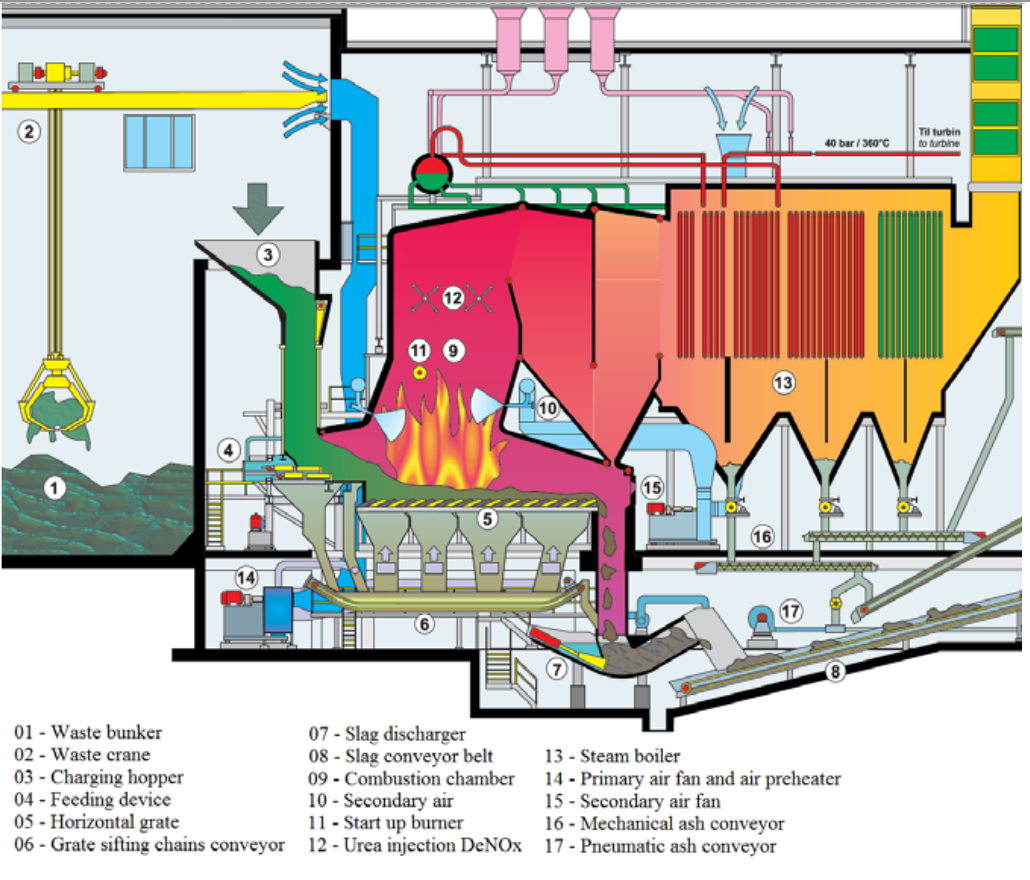
\includegraphics[width=.7\textwidth]{img/plant_overview.png}
%     \caption{Plant-overwiev}
%     \label{fig:plant_overwiev}
% \end{figure}
  

% \subsection{The combustion-process}
% % \todo[inline]{Rather have a general description of the process first, and then go in detail here}
% Even though the grate is ideally supposed to be divided into three parts, these separations are not necessarily as exact as one might hope. \todo[inline]{Add a picture, showing the post-combustion(?)} Additionally, the grate is a mass-transfer, based on the grate-speed, and the flow of flue gas is a fluid flow with potentially some heat exchange, turbulent flows and secondary combustion occurring in the gas. If the system were to be represented by ODEs (Ordinary Differential Equations), it would require infinitely many states. As a result, some kind of simplification is needed. In \cite{waste_prof}, two different first principles models were proposed. In this thesis, the second of those models will be used to get an intuitive understanding of the process. In that model, it was assumed that the combustion chamber could be modelled as a perfectly mixed system with one mass-flow \(\phi_{w,in}\) that goes into it, and two mass-flows \( \phi_{out} \) and \(\phi_{fg}\) that goes out from it, representing the ash and the flue gas respectively. Furthermore, it was assumed that the part of the waste that is capable of burning can be described as some generic combination of Carbon, Hydrogen and Oxygen \(C H_y O_z\), where the ratios may change with time. The fraction of total waste-flow entering the combustion chamber, which is combustible is denoted as \(X_{C H_y O_z}\), while the fraction which can not burn, nor evaporate is denoted \(X_{inert}\). \cite{waste_prof} assumes that all combustible material in the combustion chamber is burned. As a result, the mass-balance for the mass of inert material in the combustion chamber can be written as in Equation \ref{eq:m_inert_balance}.
% \begin{align}
%     \frac{d M_{inert}}{dt } = X_{inert}\phi_{w,in} - \phi_{out}
%     \label{eq:m_inert_balance}
% \end{align}{}
% \noindent
% If the reaction speed at which the waste burns is given by \(Ra\), then the mass balance for \(M_{CH_y O_z}\) can be written as.

% \begin{align}
% \frac{d M_{CH_y O_z}}{dt} = X_{CH_y O_z} \phi_{w,in} + Ra M_{CH_y O_z}
% \end{align}
% \noindent
% In practice, it may not be the case that all material is burned up, but assuming complete combustion simplifies the equations needed to control the system greatly. Additionally, if there are considerable effects due to incomplete combustion, the system is far from its normal region of operation. In those cases, another controller is most likely better suited for stabilizing the plant in what might essentially be an emergency.

% \noindent
% The expression used to model \( \phi_{out}\) should ideally be a time-delayed version of \(X_{inert}\phi_{in}\), where the time-delay may change depending on the grate-speed. There are several ways to model the dynamics of \(\phi_{out}\). The one proposed in \cite{waste_prof} is to use the expression 
% \begin{align}
%   \phi_{out} = C_{\phi_{out}}a M_{inert}
%   \label{eq:first_order_mass_out}
% \end{align}
% Which will be the same as using a first-order filter to simulate a time-delay. A more precise model would be to set \(l_g\) to be the length of the grate, and \(v_g\) to be the velocity which the waste would move. The resulting expression for \(\phi_{out}\) will be
% \begin{align}
%   \phi_{out} = - \frac{l_g}{v_g} \left( M_{inert} \right)
% \end{align}

% More precise approximation of time-delays, with regards to stability analysis, can be found by using padé-approximations, but that will not make it possible to describe a system with variable grate speed. \todo[inline]{Reference or better formulation}

% \noindent
% The solution proposed in \cite{waste_prof} was to lump the entire combustion chamber into one system that is assumed to be perfectly mixed. Additionally, it is assumed that how combustible material and moisture are mixed within the waste does not matter as much as the quantity. Therefore it is assumed that the moisture can be described as a separate mass-stream. Similarly, it is assumed that the non-moisture part can be described as a single mass-stream, which is a combination between the inert materials and the burnable materials. Take note that this mass is still called $M_{comb}$, even though nor all of it can be burned. As a result, the masses $M \left[ kg \right]$ can be described by mass-flows $\phi\left[ \frac{kg}{s} \right]$, reaction-rates and ratios $X\left[ \frac{kg}{kg} \right]$ for describing what the waste from the ram is composed of. The resulting equation for $M_{mois}$ is given by \ref{eq:mosture_mass_rate}



% \begin{align}
%   \frac{d M_{mois}}{dt} = X_{mois} \phi_{w,in} - k_{evap}a M_{mois}
%   \label{eq:mosture_mass_rate}
% \end{align}


% \noindent
% Where $ M_{mois}\left[ kg \right]$ is the mass of all moisture in the combustion chamber. $\phi_{w,in} \left[ \frac{kg}{s} \right]$ is the mass-flow of waste that is pushed on the grate by the ram. $X_{mois} \left[ \frac{kg}{kg} \right]$ represent the fraction of the waste that is moisture. Meanwhile, $k_{evap} \cdot a$ represents the rate which the mosture evaporates. The corresponding equation for the mass of the combustibles in the combustion chamber is given by Equation \ref{eq:comb_mass_balance}. 


% \begin{equation}
%   \frac{d M_{comb}}{dt }= X_{comb} \phi_{w,in} - \phi_{out} - RaM_{comb}
%   \label{eq:comb_mass_balance}
% \end{equation}

% \noindent
% $M_{comb}$ and $X_{comb}$ work similarly as in Equation \ref{eq:mosture_mass_rate}, but for the combination of combustible materials and the inert material. $R \cdot a\left[ \frac{1}{s} \right]$ represents the rate which the material burns with. Finally, there also exists a variable $X_{inert} \le X_{comb}$, which represents the fraction of the waste that will not burn or evaporate. The correct method for modelling mass-flow of unburned material $\phi_{out} \left[ \frac{kg}{s} \right]$ would be with a time-delay between input and the output. In the simplified model, the time-delay is removed, and is simply given by Equation \ref{eq:simple_mass_out}. For something slightly more complex, Equation \ref{eq:first_order_mass_out} can be used. 

% \begin{align}
%   \phi_{out} = X_{inert} \phi_{w, in}
%   \label{eq:simple_mass_out}
% \end{align}


% \noindent
% The differential equation which describes how the temperature of the solid waste in the combustion chamber is quite complex and depends on several new variables: 
% \begin{itemize}
%   \item $C_{comb} [\frac{J}{kg K}]$ : Specific heat-capacity for combustibles
%   \item $C_{p,fg} \left[ \frac{J}{kg K} \right]$: Specific heat-capacity of the flue gas
%   \item $T_s \left[ K \right]$: The temperature of the solid-state waste in the combustion chamber
%   \item $T_{w,in} \left[ K \right]$ Temperature of waste before it enters the combustion chamber. 
%   \item $\Delta H_{comb} \left[ \frac{J}{kg} \right]$ : Combustion entalpy
%   \item $X_{\Delta H_{comb}} \left[ - \right]$ : Fraction of $\Delta H_{comb}$ that goes into heating up the solid-state in the combuston chamber
%   \item $\Delta H_{evap}$ is the evaporation entalpy
%   \item  $\sigma = 5.6.7051 \cdot 10^{-8} \left[ \frac{W}{m^2 K^4 } \right]$ is the Stefan-Bolzmann constant
%   \item  $A_s \left[ m^2 \right]$ is the area where the solid-state and the gas exchange energy through radiation
%   \item $\epsilon_{gt} \left[ - \right]$ Flue gas emissitivity-factor
%   \item $\alpha_{gt} \left[ - \right]$: Waste absorbtivity-factor
% \end{itemize}
% The resulting temperature balance for the solid-state in the combustion-chamber becomes 
% \begin{equation}
%   \begin{split}
%     \left( C_{p, comb}M_{comb} + C_{p, mois}M_{mois} \right) \dot{T_s} =  & \left(  C_{p, comb}X_{comb} + C_{p, mois}X_{mois}  \right) \\
%     \cdot &\phi_{w,in} \left( T_{w,in} - T_s \right)\\
%     + & C_{p,fg}\phi_{prim}\left( T_{prim} - T_s \right)\\
%     + & X_{\Delta H_{comb}}R a M_{comb} \Delta H_{comb}\\
%     + & k _{evap} a M _{mois} \Delta H _{evap} \\
%     + &\sigma A_s \left( \epsilon_{gt}T_g^4 - \alpha_{gt}T_s^4 \right)
%   \end{split}
% \end{equation}

% \noindent
% The two terms from the first three lines come from energy transfer due to the mass-flows to and from the solid-state. The term from the third line comes directly from the energy transfer from the combustion, and the fourth line is similar, but it is the loss from evaporation. The last line comes from the exchange of radiation between the solid-state and the flue gas. 
% \noindent
% The combustion  $Ra$ can be somewhat tricky to model, due to the varying composition of the waste, as well as the uncertainties that come from the varying shape and the aerodynamics. If $M_{O_2} = 2 \frac{16}{1000}\left[ \frac{kg}{mol} \right]$ is the molar mass of oxygen and  $Y_{O_2,in} \left[ \frac{mol}{m^3} \right]$ is the concentration of oxygen in the primary airflow, then there is a simplified formula for the reaction rate $R$

% \begin{align}
%   R = \left( \frac{1}{\frac{1}{k_d}+ \frac{1}{k_o e^{\frac{-E_g}{R_g T_s}}}} \right) \left( \frac{Y_{O_2,in  } M_{O_2}}{v_{O_2} } \right)
% \end{align}

% This formula is not necessarily correct either, according to \cite{waste_prof}, it does seem to work empirically. Furthermore, the thesis also shows that, since $k_d << k_0 e^{\frac{-E_g}{R_g T_s}}$ in most cases, the formula can be simplified into: 
% \begin{align}
%   R = k_d \left( \frac{Y_{O_2,in}M_{O_2}}{v_{O_2}} \right)
% \end{align}

% \noindent
% The temperature of the flue gas has a similar differential equation. In \cite{waste_prof}, it is mentioned that the gas-phase has a far lower heat-capacity than the solid phase. The temperature will converge a lot faster than the temperature of the solid state. In \cite{waste_prof}, it is proposed that it happens so fast that the dynamics can be ignored. The resulting equation becomes: 

% \begin{align}
%   \begin{split}
%   0 = &C_{p,fg}\phi_{fg,in} \left( T_s-T_g \right) + C_{p,fg}\phi_{sec} \left( T_{sec}-T_g \right) +\\
%   &C_{p,fg} \phi_{rec} \left( T_{rec} - T_g  \right)+ C_{p, fg}\phi_{leak}\left( T_{leak}- T_g \right) +\\
%   &\left( 1 - X_{\Delta H_{CH_y O_z}} \right) R a M_{CH_y O_z} \Delta H_{CH_y O_z}+\\
%   &\sigma A_s \left( \alpha_{gt}T_s^4 - \epsilon_{gt}T_g^4 \right)
%   \end{split}
% \end{align}
% \todo[inline]{The phi-s were mass-flows, not molar flows}
% \subsection{Mass-balances in the combustion process}
% When calculating the concentration of \(O_2\), \(CO_2\) and \(N_2\) in the flue gas, mass-balances between the inputs to the combustion and the molar flow of the substances can be used to find the relations between the waste and the flue gas. \(\phi_{O_2,fg, in}\) is the mass-flow of \(O_2\) that is added to the flue gas as a result of the combustion. \(\phi_{CO_2, fg,in}\) and \(\phi_{N_2, fg, in} \) are the same for \(CO_2\) and nitrogen. \(MM_{O_2}\) is the molar mass of oxygen, while $\eta_c$ is the fraction of carbon that goes into the flue gas, and not into the solid state. The resulting equations, describing the mass-flows are: 
% \begin{align}
%   \phi_{O_2,fg, in} = X_{O_2, air}\phi_{prim} - \frac{1}{2}\left( 2 \eta_c + \frac{1}{2}y - z \right)\phi_{CH_y O_z}
% \end{align}
% \begin{align}
%   \phi_{CO_2, fg,in} = \eta_C \left( \frac{M M_{CO_2}}{M M_{C H_y O_z}} \right)\phi_{C H_y O_z}
% \end{align}
% \begin{align}
%   \phi_{N_2, fg, in} = X_{N_2,air}\phi_{prim}
% \end{align}

% The actual mass flow of the flue gas is instead given as the sum of \(\phi_{fg, in}\), as well as the secondary air \(\phi_{sec}\), the leakage air \(\phi_{leak}\) and the recycled air \(\phi_{recirc}\). As a result, mass flows, like water become
% \begin{align}
%   \phi_{H_2O,fg} \cdot \left(  \phi_{fg} - \phi_{recirc} \right) = \phi_{H_2 O, fg, in} + X_{H_2 O, air} \left( \phi_{sec}+ \phi_{leak}  \right)
% \end{align}

% % The same will also be done for any moisture. Meanwhile, the combustible is assumed lumped similarly. The only difference is that the ratio between $C$, $O$ and $H$ is assumed to be variable, and such that the waste is described by$C Hsimilar\todo{Say something about the simplifications that are being made}

